% Options for packages loaded elsewhere
\PassOptionsToPackage{unicode}{hyperref}
\PassOptionsToPackage{hyphens}{url}
%
\documentclass[
]{ctexart}
\usepackage{amsmath,amssymb}
\usepackage{lmodern}
\usepackage{ifxetex,ifluatex}
\ifnum 0\ifxetex 1\fi\ifluatex 1\fi=0 % if pdftex
  \usepackage[T1]{fontenc}
  \usepackage[utf8]{inputenc}
  \usepackage{textcomp} % provide euro and other symbols
\else % if luatex or xetex
  \usepackage{unicode-math}
  \defaultfontfeatures{Scale=MatchLowercase}
  \defaultfontfeatures[\rmfamily]{Ligatures=TeX,Scale=1}
  \setmonofont[]{Fira Mono}
\fi
% Use upquote if available, for straight quotes in verbatim environments
\IfFileExists{upquote.sty}{\usepackage{upquote}}{}
\IfFileExists{microtype.sty}{% use microtype if available
  \usepackage[]{microtype}
  \UseMicrotypeSet[protrusion]{basicmath} % disable protrusion for tt fonts
}{}
\makeatletter
\@ifundefined{KOMAClassName}{% if non-KOMA class
  \IfFileExists{parskip.sty}{%
    \usepackage{parskip}
  }{% else
    \setlength{\parindent}{0pt}
    \setlength{\parskip}{6pt plus 2pt minus 1pt}}
}{% if KOMA class
  \KOMAoptions{parskip=half}}
\makeatother
\usepackage{xcolor}
\IfFileExists{xurl.sty}{\usepackage{xurl}}{} % add URL line breaks if available
\IfFileExists{bookmark.sty}{\usepackage{bookmark}}{\usepackage{hyperref}}
\hypersetup{
  pdftitle={Exploratory Data Analysis},
  hidelinks,
  pdfcreator={LaTeX via pandoc}}
\urlstyle{same} % disable monospaced font for URLs
\usepackage[left=2cm, right=2cm, top=2.5cm, bottom=2.5cm]{geometry}
\usepackage{color}
\usepackage{fancyvrb}
\newcommand{\VerbBar}{|}
\newcommand{\VERB}{\Verb[commandchars=\\\{\}]}
\DefineVerbatimEnvironment{Highlighting}{Verbatim}{commandchars=\\\{\}}
% Add ',fontsize=\small' for more characters per line
\usepackage{framed}
\definecolor{shadecolor}{RGB}{248,248,248}
\newenvironment{Shaded}{\begin{snugshade}}{\end{snugshade}}
\newcommand{\AlertTok}[1]{\textcolor[rgb]{0.94,0.16,0.16}{#1}}
\newcommand{\AnnotationTok}[1]{\textcolor[rgb]{0.56,0.35,0.01}{\textbf{\textit{#1}}}}
\newcommand{\AttributeTok}[1]{\textcolor[rgb]{0.77,0.63,0.00}{#1}}
\newcommand{\BaseNTok}[1]{\textcolor[rgb]{0.00,0.00,0.81}{#1}}
\newcommand{\BuiltInTok}[1]{#1}
\newcommand{\CharTok}[1]{\textcolor[rgb]{0.31,0.60,0.02}{#1}}
\newcommand{\CommentTok}[1]{\textcolor[rgb]{0.56,0.35,0.01}{\textit{#1}}}
\newcommand{\CommentVarTok}[1]{\textcolor[rgb]{0.56,0.35,0.01}{\textbf{\textit{#1}}}}
\newcommand{\ConstantTok}[1]{\textcolor[rgb]{0.00,0.00,0.00}{#1}}
\newcommand{\ControlFlowTok}[1]{\textcolor[rgb]{0.13,0.29,0.53}{\textbf{#1}}}
\newcommand{\DataTypeTok}[1]{\textcolor[rgb]{0.13,0.29,0.53}{#1}}
\newcommand{\DecValTok}[1]{\textcolor[rgb]{0.00,0.00,0.81}{#1}}
\newcommand{\DocumentationTok}[1]{\textcolor[rgb]{0.56,0.35,0.01}{\textbf{\textit{#1}}}}
\newcommand{\ErrorTok}[1]{\textcolor[rgb]{0.64,0.00,0.00}{\textbf{#1}}}
\newcommand{\ExtensionTok}[1]{#1}
\newcommand{\FloatTok}[1]{\textcolor[rgb]{0.00,0.00,0.81}{#1}}
\newcommand{\FunctionTok}[1]{\textcolor[rgb]{0.00,0.00,0.00}{#1}}
\newcommand{\ImportTok}[1]{#1}
\newcommand{\InformationTok}[1]{\textcolor[rgb]{0.56,0.35,0.01}{\textbf{\textit{#1}}}}
\newcommand{\KeywordTok}[1]{\textcolor[rgb]{0.13,0.29,0.53}{\textbf{#1}}}
\newcommand{\NormalTok}[1]{#1}
\newcommand{\OperatorTok}[1]{\textcolor[rgb]{0.81,0.36,0.00}{\textbf{#1}}}
\newcommand{\OtherTok}[1]{\textcolor[rgb]{0.56,0.35,0.01}{#1}}
\newcommand{\PreprocessorTok}[1]{\textcolor[rgb]{0.56,0.35,0.01}{\textit{#1}}}
\newcommand{\RegionMarkerTok}[1]{#1}
\newcommand{\SpecialCharTok}[1]{\textcolor[rgb]{0.00,0.00,0.00}{#1}}
\newcommand{\SpecialStringTok}[1]{\textcolor[rgb]{0.31,0.60,0.02}{#1}}
\newcommand{\StringTok}[1]{\textcolor[rgb]{0.31,0.60,0.02}{#1}}
\newcommand{\VariableTok}[1]{\textcolor[rgb]{0.00,0.00,0.00}{#1}}
\newcommand{\VerbatimStringTok}[1]{\textcolor[rgb]{0.31,0.60,0.02}{#1}}
\newcommand{\WarningTok}[1]{\textcolor[rgb]{0.56,0.35,0.01}{\textbf{\textit{#1}}}}
\usepackage{graphicx}
\makeatletter
\def\maxwidth{\ifdim\Gin@nat@width>\linewidth\linewidth\else\Gin@nat@width\fi}
\def\maxheight{\ifdim\Gin@nat@height>\textheight\textheight\else\Gin@nat@height\fi}
\makeatother
% Scale images if necessary, so that they will not overflow the page
% margins by default, and it is still possible to overwrite the defaults
% using explicit options in \includegraphics[width, height, ...]{}
\setkeys{Gin}{width=\maxwidth,height=\maxheight,keepaspectratio}
% Set default figure placement to htbp
\makeatletter
\def\fps@figure{htbp}
\makeatother
\setlength{\emergencystretch}{3em} % prevent overfull lines
\providecommand{\tightlist}{%
  \setlength{\itemsep}{0pt}\setlength{\parskip}{0pt}}
\setcounter{secnumdepth}{5}
\let\oldhref\href
\renewcommand{\href}[2]{\oldhref{#1}{\textcolor{blue}{\underline{#2}}}}

\let\oldhyperlink\hyperlink
\renewcommand{\hyperlink}[2]{\oldhyperlink{#1}{\textcolor{red}{\underline{#2}}}}
\ifluatex
  \usepackage{selnolig}  % disable illegal ligatures
\fi
\newlength{\cslhangindent}
\setlength{\cslhangindent}{1.5em}
\newlength{\csllabelwidth}
\setlength{\csllabelwidth}{3em}
\newenvironment{CSLReferences}[2] % #1 hanging-ident, #2 entry spacing
 {% don't indent paragraphs
  \setlength{\parindent}{0pt}
  % turn on hanging indent if param 1 is 1
  \ifodd #1 \everypar{\setlength{\hangindent}{\cslhangindent}}\ignorespaces\fi
  % set entry spacing
  \ifnum #2 > 0
  \setlength{\parskip}{#2\baselineskip}
  \fi
 }%
 {}
\usepackage{calc}
\newcommand{\CSLBlock}[1]{#1\hfill\break}
\newcommand{\CSLLeftMargin}[1]{\parbox[t]{\csllabelwidth}{#1}}
\newcommand{\CSLRightInline}[1]{\parbox[t]{\linewidth - \csllabelwidth}{#1}\break}
\newcommand{\CSLIndent}[1]{\hspace{\cslhangindent}#1}

\title{Exploratory Data Analysis}
\usepackage{etoolbox}
\makeatletter
\providecommand{\subtitle}[1]{% add subtitle to \maketitle
  \apptocmd{\@title}{\par {\large #1 \par}}{}{}
}
\makeatother
\subtitle{可重复性报告 - 作为报告草稿}
\author{}
\date{\vspace{-2.5em}}

\begin{document}
\maketitle

{
\setcounter{tocdepth}{2}
\tableofcontents
}
\hypertarget{ux73afux5883}{%
\section{环境}\label{ux73afux5883}}

\hypertarget{r-info}{%
\subsection{R info}\label{r-info}}

\begin{Shaded}
\begin{Highlighting}[]
\NormalTok{xfun}\SpecialCharTok{::}\FunctionTok{session\_info}\NormalTok{(}
        \AttributeTok{packages =} \FunctionTok{c}\NormalTok{(}
                \StringTok{"readr"}\NormalTok{, }\StringTok{"tidyr"}\NormalTok{, }\StringTok{"stringr"}\NormalTok{, }\StringTok{"dplyr"}\NormalTok{, }\StringTok{"purrr"}\NormalTok{,}
                \StringTok{"tidyverse"}\NormalTok{, }\StringTok{"lubridate"}\NormalTok{, }\StringTok{"mice"}\NormalTok{,}
                \StringTok{"ggplot2"}\NormalTok{, }\StringTok{"ggdag"}\NormalTok{, }\StringTok{"showtext"}\NormalTok{, }\StringTok{"VIM"}
\NormalTok{        ), }\AttributeTok{dependencies =} \ConstantTok{FALSE}
\NormalTok{)}
\end{Highlighting}
\end{Shaded}

\begin{verbatim}
R version 4.1.0 (2021-05-18)
Platform: x86_64-pc-linux-gnu (64-bit)
Running under: Ubuntu 20.04.2 LTS

Locale:
  LC_CTYPE=zh_CN.UTF-8       LC_NUMERIC=C              
  LC_TIME=zh_CN.UTF-8        LC_COLLATE=zh_CN.UTF-8    
  LC_MONETARY=zh_CN.UTF-8    LC_MESSAGES=zh_CN.UTF-8   
  LC_PAPER=zh_CN.UTF-8       LC_NAME=C                 
  LC_ADDRESS=C               LC_TELEPHONE=C            
  LC_MEASUREMENT=zh_CN.UTF-8 LC_IDENTIFICATION=C       

Package version:
  dplyr_1.0.6      ggdag_0.2.3      ggplot2_3.3.3    lubridate_1.7.10
  mice_3.13.0      purrr_0.3.4      readr_1.4.0      showtext_0.9-2  
  stringr_1.4.0    tidyr_1.1.3      tidyverse_1.3.1  VIM_6.1.0       
\end{verbatim}

\hypertarget{python-info}{%
\subsection{python info}\label{python-info}}

// TODO

\hypertarget{ux5206ux6790}{%
\section{分析}\label{ux5206ux6790}}

\hypertarget{the-workflow}{%
\subsection{The Workflow}\label{the-workflow}}

\begin{figure}
\centering
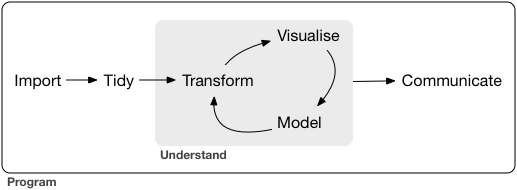
\includegraphics{workflow.png}
\caption[The Data Science Workflow]{The Data Science
Workflow\footnotemark{}}
\end{figure}
\footnotetext{This picture is from
  \href{https://r4ds.had.co.nz/introduction.html}{R for Data Science} by
  Hadley Wickham and Garrett Grolemund, released under
  \href{http://creativecommons.org/licenses/by-nc-nd/3.0/us/}{CC
  BY-NC-ND 3.0 US}.}

\hypertarget{import}{%
\subsection{Import}\label{import}}

// 需要数据集的完整描述和获取方式

// TODO - \textbf{R. Li}

\hypertarget{tidy}{%
\subsection{Tidy}\label{tidy}}

\begin{Shaded}
\begin{Highlighting}[]
\NormalTok{raw\_df }\OtherTok{\textless{}{-}} \FunctionTok{read\_csv}\NormalTok{(}\StringTok{"./data/investment/FDI\_untidy.csv"}\NormalTok{)}

\NormalTok{process }\OtherTok{\textless{}{-}} \ControlFlowTok{function}\NormalTok{(raw\_df) \{}
\NormalTok{  simplified\_df }\OtherTok{\textless{}{-}}\NormalTok{ raw\_df }\SpecialCharTok{\%\textgreater{}\%}
    \FunctionTok{filter}\NormalTok{(X1 }\SpecialCharTok{\%\textgreater{}\%} \FunctionTok{str\_detect}\NormalTok{(}\StringTok{"\^{}}\SpecialCharTok{\textbackslash{}\textbackslash{}}\StringTok{d"}\NormalTok{)) }\SpecialCharTok{\%\textgreater{}\%}
    \FunctionTok{rename}\NormalTok{(时间 }\OtherTok{=}\NormalTok{ X1)}

\NormalTok{  fliped\_df }\OtherTok{\textless{}{-}}\NormalTok{ simplified\_df }\SpecialCharTok{\%\textgreater{}\%}
    \FunctionTok{pivot\_longer}\NormalTok{(}\FunctionTok{c}\NormalTok{(}\SpecialCharTok{{-}}\NormalTok{时间), }\AttributeTok{names\_to =} \StringTok{"observation"}\NormalTok{, }\AttributeTok{values\_to =} \StringTok{"val"}\NormalTok{)}

\NormalTok{  stdize }\OtherTok{\textless{}{-}} \ControlFlowTok{function}\NormalTok{(str) \{}
\NormalTok{    str }\SpecialCharTok{\%\textgreater{}\%}
      \FunctionTok{str\_replace}\NormalTok{(}\AttributeTok{pattern =} \StringTok{"(.*):(总计|一带一路)"}\NormalTok{, }\AttributeTok{replacement =} \StringTok{"}\SpecialCharTok{\textbackslash{}\textbackslash{}}\StringTok{1/}\SpecialCharTok{\textbackslash{}\textbackslash{}}\StringTok{2/}\SpecialCharTok{\textbackslash{}\textbackslash{}}\StringTok{2"}\NormalTok{) }\SpecialCharTok{\%\textgreater{}\%}
      \FunctionTok{str\_replace}\NormalTok{(}\AttributeTok{pattern =} \StringTok{"::"}\NormalTok{, }\AttributeTok{replacement =} \StringTok{":"}\NormalTok{) }\SpecialCharTok{\%\textgreater{}\%}
      \FunctionTok{str\_replace}\NormalTok{(}\AttributeTok{pattern =} \StringTok{"(.*):(.*洲):*(.*)"}\NormalTok{, }\AttributeTok{replacement =} \StringTok{"}\SpecialCharTok{\textbackslash{}\textbackslash{}}\StringTok{1/}\SpecialCharTok{\textbackslash{}\textbackslash{}}\StringTok{2/}\SpecialCharTok{\textbackslash{}\textbackslash{}}\StringTok{3"}\NormalTok{)}
\NormalTok{  \}}

\NormalTok{  sep\_df }\OtherTok{\textless{}{-}}\NormalTok{ fliped\_df }\SpecialCharTok{\%\textgreater{}\%}
    \FunctionTok{mutate}\NormalTok{(}\AttributeTok{observation =}\NormalTok{ observation }\SpecialCharTok{\%\textgreater{}\%} \FunctionTok{stdize}\NormalTok{()) }\SpecialCharTok{\%\textgreater{}\%}
    \FunctionTok{separate}\NormalTok{(}\AttributeTok{col =} \StringTok{"observation"}\NormalTok{, }\AttributeTok{into =} \FunctionTok{c}\NormalTok{(}\StringTok{"type"}\NormalTok{, }\StringTok{"地区"}\NormalTok{, }\StringTok{"国家"}\NormalTok{), }\AttributeTok{sep =} \StringTok{"/"}\NormalTok{)}

\NormalTok{  df }\OtherTok{\textless{}{-}}\NormalTok{ sep\_df }\SpecialCharTok{\%\textgreater{}\%} \FunctionTok{spread}\NormalTok{(}\AttributeTok{key =} \StringTok{"type"}\NormalTok{, }\AttributeTok{value =} \StringTok{"val"}\NormalTok{)}
\NormalTok{\}}

\NormalTok{raw\_df }\SpecialCharTok{\%\textgreater{}\%}
  \FunctionTok{process}\NormalTok{() }\SpecialCharTok{\%\textgreater{}\%}
  \FunctionTok{write\_csv}\NormalTok{(}\StringTok{"./data/investment/FDI\_tidy.csv"}\NormalTok{)}

\NormalTok{cont }\OtherTok{\textless{}{-}}\NormalTok{ raw\_df }\SpecialCharTok{\%\textgreater{}\%}
  \FunctionTok{filter}\NormalTok{(X1 }\SpecialCharTok{==} \StringTok{"状态"}\NormalTok{) }\SpecialCharTok{\%\textgreater{}\%}
  \FunctionTok{as\_vector}\NormalTok{() }\SpecialCharTok{\%\textgreater{}\%}
\NormalTok{  .[. }\SpecialCharTok{==} \StringTok{"继续"}\NormalTok{] }\SpecialCharTok{\%\textgreater{}\%}
  \FunctionTok{names}\NormalTok{()}
\NormalTok{raw\_df }\SpecialCharTok{\%\textgreater{}\%}
  \FunctionTok{select}\NormalTok{(X1, }\FunctionTok{all\_of}\NormalTok{(cont)) }\SpecialCharTok{\%\textgreater{}\%}
  \FunctionTok{process}\NormalTok{() }\SpecialCharTok{\%\textgreater{}\%}
  \FunctionTok{write\_csv}\NormalTok{(}\StringTok{"./data/investment/FDI\_tidy\_cont.csv"}\NormalTok{)}
\end{Highlighting}
\end{Shaded}

\begin{Shaded}
\begin{Highlighting}[]
\NormalTok{raw\_df }\OtherTok{\textless{}{-}} \FunctionTok{read\_csv}\NormalTok{(}
  \AttributeTok{file =} \StringTok{"./data/investment/FDI\_tidy\_cont.csv"}\NormalTok{,}
  \AttributeTok{col\_types =} \FunctionTok{cols}\NormalTok{(}
\NormalTok{    时间 }\OtherTok{=} \FunctionTok{col\_date}\NormalTok{(}\AttributeTok{format =} \StringTok{"\%m/\%Y"}\NormalTok{)}
\NormalTok{  ),}
  \AttributeTok{guess\_max =} \DecValTok{50000}
\NormalTok{)}

\NormalTok{df0 }\OtherTok{\textless{}{-}}\NormalTok{ raw\_df }\SpecialCharTok{\%\textgreater{}\%}
  \FunctionTok{filter}\NormalTok{(}\SpecialCharTok{!}\FunctionTok{is.na}\NormalTok{(国家))}

\CommentTok{\# 对外直接投资:非金融类:累计 为一带一路数据所特有}
\NormalTok{OBOR\_col }\OtherTok{\textless{}{-}} \StringTok{"对外直接投资:非金融类:累计"}

\NormalTok{df }\OtherTok{\textless{}{-}}\NormalTok{ df0 }\SpecialCharTok{\%\textgreater{}\%}
  \FunctionTok{filter}\NormalTok{(国家 }\SpecialCharTok{!=} \StringTok{"一带一路"} \SpecialCharTok{\&}\NormalTok{ 国家 }\SpecialCharTok{!=} \StringTok{"总计"}\NormalTok{) }\SpecialCharTok{\%\textgreater{}\%}
  \FunctionTok{select}\NormalTok{(}\SpecialCharTok{{-}}\FunctionTok{all\_of}\NormalTok{(OBOR\_col))}

\NormalTok{df }\OtherTok{\textless{}{-}}\NormalTok{ df }\SpecialCharTok{\%\textgreater{}\%}
  \FunctionTok{filter}\NormalTok{(}\FunctionTok{month}\NormalTok{(时间) }\SpecialCharTok{==} \DecValTok{12}\NormalTok{) }\SpecialCharTok{\%\textgreater{}\%}
  \FunctionTok{mutate}\NormalTok{(年份 }\OtherTok{=} \FunctionTok{as.integer}\NormalTok{(}\FunctionTok{year}\NormalTok{(时间)), }\AttributeTok{.keep =} \StringTok{"unused"}\NormalTok{, }\AttributeTok{.before =} \DecValTok{1}\NormalTok{) }\SpecialCharTok{\%\textgreater{}\%}
  \FunctionTok{filter}\NormalTok{(年份 }\SpecialCharTok{\textgreater{}=} \DecValTok{2002}\NormalTok{)}

\NormalTok{df }\OtherTok{\textless{}{-}}\NormalTok{ df }\SpecialCharTok{\%\textgreater{}\%}
  \FunctionTok{select}\NormalTok{(}\FunctionTok{names}\NormalTok{(df) }\SpecialCharTok{\%\textgreater{}\%} \FunctionTok{str\_subset}\NormalTok{(}\AttributeTok{pattern =} \StringTok{"投资(和其他)*$"}\NormalTok{, }\AttributeTok{negate =} \ConstantTok{TRUE}\NormalTok{)) }\SpecialCharTok{\%\textgreater{}\%}
  \FunctionTok{filter}\NormalTok{(}\SpecialCharTok{!}\FunctionTok{is.na}\NormalTok{(}\StringTok{\textasciigrave{}}\AttributeTok{对外直接投资:截至累计}\StringTok{\textasciigrave{}}\NormalTok{))}

\NormalTok{df }\SpecialCharTok{\%\textgreater{}\%} \FunctionTok{write\_csv}\NormalTok{(}\AttributeTok{file =} \StringTok{"./data/investment/FDI\_useful.csv"}\NormalTok{)}

\NormalTok{df1 }\OtherTok{\textless{}{-}}\NormalTok{ df0 }\SpecialCharTok{\%\textgreater{}\%}
  \FunctionTok{filter}\NormalTok{(国家 }\SpecialCharTok{==} \StringTok{"一带一路"} \SpecialCharTok{\&} \SpecialCharTok{!}\FunctionTok{is.na}\NormalTok{(.[OBOR\_col])) }\SpecialCharTok{\%\textgreater{}\%}
  \FunctionTok{select}\NormalTok{(时间, }\FunctionTok{all\_of}\NormalTok{(OBOR\_col)) }\SpecialCharTok{\%\textgreater{}\%}
  \FunctionTok{mutate}\NormalTok{(}
\NormalTok{    年份 }\OtherTok{=} \FunctionTok{as.integer}\NormalTok{(}\FunctionTok{year}\NormalTok{(时间)),}
\NormalTok{    月份 }\OtherTok{=} \FunctionTok{as.integer}\NormalTok{(}\FunctionTok{month}\NormalTok{(时间)),}
    \AttributeTok{.keep =} \StringTok{"unused"}\NormalTok{, }\AttributeTok{.before =} \DecValTok{1}\NormalTok{) }\SpecialCharTok{\%\textgreater{}\%}
  \FunctionTok{arrange}\NormalTok{(年份, 月份)}

\NormalTok{df1 }\SpecialCharTok{\%\textgreater{}\%} \FunctionTok{write\_csv}\NormalTok{(}\AttributeTok{file =} \StringTok{"./data/investment/FDI\_OBOR.csv"}\NormalTok{)}
\end{Highlighting}
\end{Shaded}

\hypertarget{understand}{%
\subsection{Understand}\label{understand}}

我们的数据模型非常简单,如图所示:

\begin{figure}

{\centering \includegraphics[width=0.65\linewidth,height=0.6\textheight]{doc_files/figure-latex/unnamed-chunk-5-1} 

}

\caption{数据模型示意图}\label{fig:unnamed-chunk-5}
\end{figure}

此图是有向无环图(Directed acyclic graph, DAG),边代表因果作用.

我们利用(Chernozhukov et al.,
2021)\textsuperscript{{[}1{]}}的方法进行分析.

首先注意到数据集中存在许多缺失数据:

\begin{figure}

{\centering \includegraphics[width=0.65\linewidth,height=0.6\textheight]{doc_files/figure-latex/unnamed-chunk-6-1} 

}

\caption{缺失数据示意图}\label{fig:unnamed-chunk-6}
\end{figure}

使用linear regression with bootstrap进行缺失数据填补.

\begin{Shaded}
\begin{Highlighting}[]
\NormalTok{fdi }\OtherTok{\textless{}{-}} \FunctionTok{read\_csv}\NormalTok{(}
  \AttributeTok{file =} \StringTok{"./data/investment/FDI\_useful.csv"}\NormalTok{,}
  \AttributeTok{col\_types =} \FunctionTok{cols}\NormalTok{(}
\NormalTok{    年份 }\OtherTok{=} \FunctionTok{col\_double}\NormalTok{(),}
\NormalTok{    国家 }\OtherTok{=} \FunctionTok{col\_factor}\NormalTok{()}
\NormalTok{  )}
\NormalTok{) }\SpecialCharTok{\%\textgreater{}\%} \FunctionTok{unite}\NormalTok{(}\AttributeTok{col =}\NormalTok{ 国家, 地区, 国家)}

\NormalTok{country\_name }\OtherTok{\textless{}{-}}\NormalTok{ fdi[[}\StringTok{"国家"}\NormalTok{]] }\SpecialCharTok{\%\textgreater{}\%} \FunctionTok{unique}\NormalTok{()}

\NormalTok{fdi\_na }\OtherTok{\textless{}{-}}\NormalTok{ fdi }\SpecialCharTok{\%\textgreater{}\%}
\NormalTok{  tidyr}\SpecialCharTok{::}\FunctionTok{complete}\NormalTok{(年份, 国家) }\SpecialCharTok{\%\textgreater{}\%}
  \FunctionTok{rename}\NormalTok{(对外直接投资 }\OtherTok{=} \StringTok{\textasciigrave{}}\AttributeTok{对外直接投资:截至累计}\StringTok{\textasciigrave{}}\NormalTok{)}

\NormalTok{fdi\_lg }\OtherTok{\textless{}{-}}\NormalTok{ fdi\_na }\SpecialCharTok{\%\textgreater{}\%}
  \FunctionTok{mutate}\NormalTok{(}\AttributeTok{lg =} \FunctionTok{log}\NormalTok{(对外直接投资), }\AttributeTok{.keep =} \StringTok{"unused"}\NormalTok{)}

\NormalTok{fill\_a\_country }\OtherTok{\textless{}{-}} \ControlFlowTok{function}\NormalTok{(.dt, .cn) \{}
\NormalTok{  res }\OtherTok{\textless{}{-}}\NormalTok{ .dt }\SpecialCharTok{\%\textgreater{}\%}
    \FunctionTok{filter}\NormalTok{(国家 }\SpecialCharTok{==}\NormalTok{ .cn) }\SpecialCharTok{\%\textgreater{}\%}
    \FunctionTok{mice}\NormalTok{(}\AttributeTok{method =} \StringTok{"norm.boot"}\NormalTok{, }\AttributeTok{m =} \DecValTok{1}\NormalTok{, }\AttributeTok{maxit =} \DecValTok{3}\NormalTok{) }\SpecialCharTok{\%\textgreater{}\%}
    \FunctionTok{complete}\NormalTok{()}
  \ControlFlowTok{if}\NormalTok{ (}\FunctionTok{any}\NormalTok{(}\FunctionTok{is.na}\NormalTok{(res}\SpecialCharTok{$}\NormalTok{lg))) \{}
\NormalTok{    non\_na }\OtherTok{\textless{}{-}} \SpecialCharTok{!}\NormalTok{(res}\SpecialCharTok{$}\NormalTok{lg }\SpecialCharTok{\%\textgreater{}\%} \FunctionTok{is.na}\NormalTok{())}
\NormalTok{    res}\SpecialCharTok{$}\NormalTok{lg }\OtherTok{\textless{}{-}}\NormalTok{ res}\SpecialCharTok{$}\NormalTok{lg[non\_na][}\DecValTok{1}\NormalTok{]}
\NormalTok{  \}}
  \FunctionTok{return}\NormalTok{(res)}
\NormalTok{\}}

\NormalTok{fdi\_filled }\OtherTok{\textless{}{-}}\NormalTok{ country\_name }\SpecialCharTok{\%\textgreater{}\%} \FunctionTok{map}\NormalTok{(}\SpecialCharTok{\textasciitilde{}}\FunctionTok{fill\_a\_country}\NormalTok{(fdi\_lg, .x))}

\NormalTok{result }\OtherTok{\textless{}{-}}\NormalTok{ fdi\_filled }\SpecialCharTok{\%\textgreater{}\%}
  \FunctionTok{reduce}\NormalTok{(rbind) }\SpecialCharTok{\%\textgreater{}\%}
  \FunctionTok{mutate}\NormalTok{(对外直接投资 }\OtherTok{=} \FunctionTok{exp}\NormalTok{(lg), }\AttributeTok{.keep =} \StringTok{"unused"}\NormalTok{) }\SpecialCharTok{\%\textgreater{}\%}
  \FunctionTok{separate}\NormalTok{(}\AttributeTok{col =}\NormalTok{ 国家, }\AttributeTok{into =} \FunctionTok{c}\NormalTok{(}\StringTok{"地区"}\NormalTok{, }\StringTok{"国家"}\NormalTok{), }\AttributeTok{sep =} \StringTok{"\_"}\NormalTok{)}

\NormalTok{result }\SpecialCharTok{\%\textgreater{}\%} \FunctionTok{write\_csv}\NormalTok{(}\StringTok{"./data/investment/FDI\_filled.csv"}\NormalTok{)}
\end{Highlighting}
\end{Shaded}

\hypertarget{communicate}{%
\subsection{Communicate}\label{communicate}}

// Use \textbf{echarts}, maybe
\href{https://github.com/pyecharts}{\textbf{pyecharts}}?

// TODO - H. Fan

\hypertarget{ux603bux7ed3}{%
\section{总结}\label{ux603bux7ed3}}

\hypertarget{ux53c2ux8003ux6587ux732e}{%
\section*{参考文献}\label{ux53c2ux8003ux6587ux732e}}
\addcontentsline{toc}{section}{参考文献}

\hypertarget{refs}{}
\begin{CSLReferences}{0}{0}
\leavevmode\hypertarget{ref-doi:10.1080ux2f01621459.2021.1920957}{}%
\CSLLeftMargin{{[}1{]} }
\CSLRightInline{CHERNOZHUKOV V, WÜTHRICH K, ZHU Y. An Exact and Robust
Conformal Inference Method for Counterfactual and Synthetic
Controls{[}J{]}. Journal of the American Statistical Association, Taylor
\& Francis, 2021, 0(ja): 1--44.}

\end{CSLReferences}

\end{document}
